
\section{Results}
\label{ss: results}

In this section, we address the research questions from Section~\ref{ss: questions} 
by applying the methodology from Section~\ref{ss: metrics}.
We apply \nbAnalyzers{} widely used PDF scanners to a total of \nbSamplesSize{} malicious PDF documents generated by the Chameleon framework and an additional \nbBenignsSize{} benign PDF documents.
The benign documents comprise train tickets, governmental documents, manuals, tutorials, and some suspicious looking PDF files that are known to be benign.
All documents used for our study will be made available as a benchmark for future work.

\subsection{RQ1: Recall and False Positives}
\label{ss: recall fps}

The following addresses RQ1, i.e., how accurately the scanners classify 
documents into malicious and benign in the presence of evasions.
We measure the recall and the false positive 
ratio of each scanner, as described in Section~\ref{ss: metrics}.
Figure~\ref{fig: recall fp ratio} shows the results.
A higher recall means that the scanner is more successful in 
identifying malicious PDF documents, despite the presence of evasions.
The figure shows that almost all studied scanners are affected by evasions, 
as their recall values are lower than 100\%.
Furthermore, we find a huge variation across the studied scanners: While 
some scanners, e.g., SAFE-PDF and AVG, identify all or most malicious documents despite 
evasions, others miss many malicious documents.
Some scanners have a recall lower than 20\%, showing that they are easily 
bypassed by evasions.

In principle, a scanner could achieve 100\% recall by labeling each document 
as malicious.
To address this potential problem, Figure~\ref{fig: recall fp ratio} also 
shows the false positive ratio of each scanner.
We find that all scanners have a false positive ratio below 15\%, except Cuckoo (17.5\%), Slayer (28.77\%), and SAFE-PDF (34.57\%).
There is no strong correlation (Pearson correlation coefficient: 36.61\%) between recall and false positive ratio.
We conclude from these results that none of the scanners tries to boost its 
recall at the cost of precision, which seems reasonable as users easily drop 
a tool if they are overwhelmed with spurious warnings.


\begin{figure*}[t]
	\begin{minipage}{0.55\textwidth}
		\hspace{-.6em}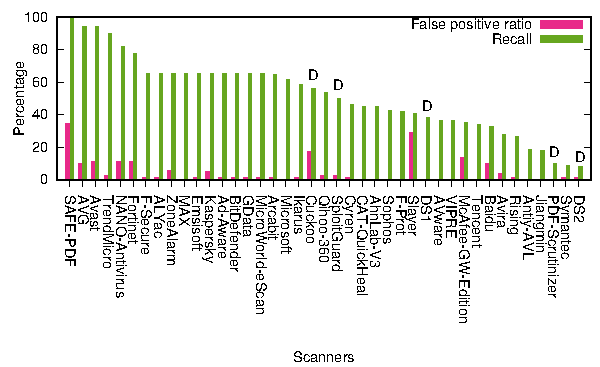
\includegraphics{figures/fp-ratio-recall}
		\captionof{figure}{Recall and false positive ratio of the studied scanners.  
			The dynamic scanners are marked with ``D''.}
		\label{fig: recall fp ratio}
	\end{minipage}
	\hfill
	\begin{minipage}{0.4\textwidth}
		\hspace{-.6em}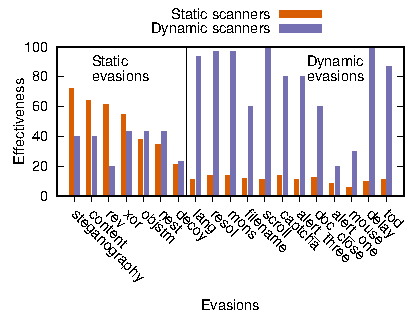
\includegraphics{figures/average-best-case-eff}
		\captionof{figure}{Effectiveness for different classes of static and 
			dynamic evasions. The results are averaged over all static 
			(red) and dynamic (blue) scanners.}
		\label{fig: best case eff}
	\end{minipage}		
\end{figure*}	


\subsection{RQ2: Evasion Effectiveness by Scanner}

To better understand the susceptibility of the scanners to static and dynamic evasions, we assess the effectiveness of evasions in bypassing specific 
scanners (RQ2).
We compute the evasion effectiveness for each 
scanner by averaging the effectiveness across all evasions.
Figures~\ref{fig: static evasions proj} and~\ref{fig: dynamic evasions proj} 
present the results for static and dynamic evasions, respectively.
A lower value indicates that a scanner is less susceptible to evasions.
The results for the static evasions in Figure~\ref{fig: static evasions 
proj} show some interesting effects.
Somewhat surprisingly, the effectiveness of 12 of the~\nbVirusTotalEngines{} VirusTotal scanners, roughly 
in the middle of the figure, is exactly the same, out of which 8 have the exact same recall, too (Figure~\ref{fig: recall fp ratio}).
A possible explanation is that multiple scanners rely on 
the same underlying decision mechanism, e.g., because one scanner queries 
another scanner as part of its decision, or because the same analysis 
algorithm is provided under several brands.
Previous, informal reports claim that some static scanners share their results~\cite{static_analyzers_share_analysis_result}, which our results 
confirm.


\begin{figure*}[tb]
	\begin{minipage}{0.55\textwidth}
		 \begin{subfigure}{\textwidth}
			  	\hspace{-.6em}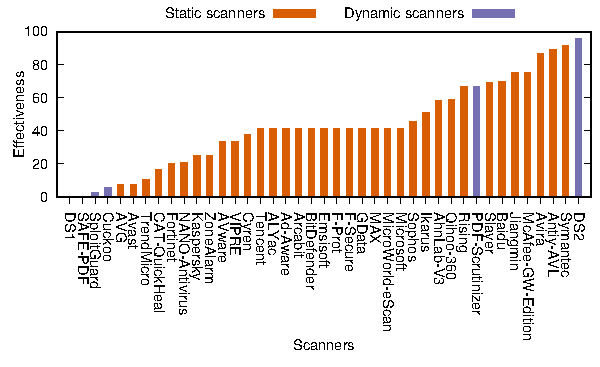
\includegraphics{figures/static-evasions-projection}
			  	\caption{Static evasions}
			  	\label{fig: static evasions proj}
		 \end{subfigure}		 
		 \begin{subfigure}{\textwidth}
			  	\hspace{-.6em}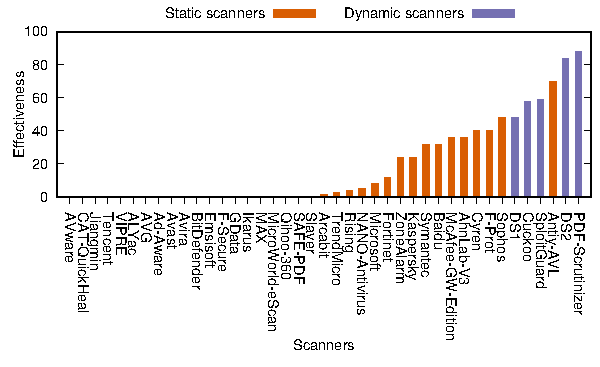
\includegraphics{figures/dynamic-evasions-projection}
			  	\caption{Dynamic evasions}
			  	\label{fig: dynamic evasions proj}
		 \end{subfigure}
		 \caption{Per-scanner effectiveness of static and dynamic evasions.}		
	\end{minipage}
	\hspace{1em}
	\begin{minipage}{0.4\linewidth}
		\begin{subfigure}[b]{\textwidth}
			\hspace*{-.6em}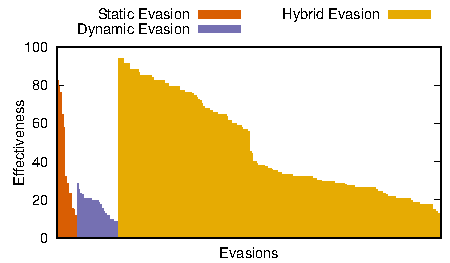
\includegraphics{figures/toolbutton-projection}
			\caption{Documents with ``Toolbutton'' exploit.}
			\label{figure:toolbutton projection}
		\end{subfigure}
		\vspace{2em}
		
		\begin{subfigure}[b]{\textwidth}
			\hspace*{-.6em}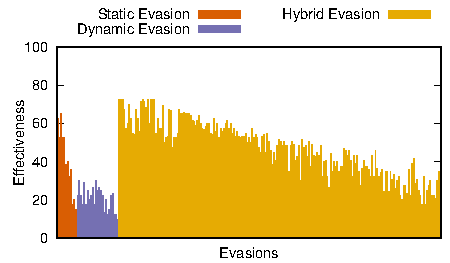
\includegraphics{figures/cooltype-projection}
			\caption{Documents with ``Cooltype'' exploit.}
			\label{figure:cooltype projection}
		\end{subfigure}
		\caption{Effectiveness of evasions for the subsets of malicious documents that use a specific exploit. Each bar corresponds to an evasion with a specific argument. The hybrid evasions, and some of the static and dynamic evasions  result from combining evasions (Section~\ref{ss: combination of evasions}).}
	\end{minipage}
\end{figure*}


Another interesting observation is that a dynamic, not a static, scanner (DS2) is the most susceptible to static evasions.
A comparison of  Figures~\ref{fig: static evasions proj} and~\ref{fig: dynamic evasions proj} shows that DS2 is highly susceptible to both dynamic and static evasions.
This finding suggests that DS2 not only uses dynamic analysis, but also 
heavily relies on static analysis techniques.

The static scanners in the right part of Figure~\ref{fig: dynamic evasions proj} are
impacted by dynamic evasions.
A likely reason is that adding an evasion changes the signature of the PDF documents, and that the scanners rely on these signatures.


\subsection{RQ3: Most Effective Evasions}
\label{ss:best-case effectiveness}

Understanding which evasions are most effective (RQ3) is important both for attackers and for developers of security scanners.
We measure the effectiveness of evasions for each scanner and then compute 
the average over all static and the average over all dynamic 
scanners.
Some evasions take arguments, e.g., the language used by the ``lang'' evasion or the xor key used by the ``xor'' evasion.
For such evasions, we try a range of arguments and report the highest observed effectiveness.

Figure~\ref{fig: best case eff} shows the results.
We sort the evasions as in Table~\ref{t:evasions}.
Overall, the results show that static scanners are much more susceptible to 
static evasions, while dynamic scanners get fooled by dynamic evasions, 
which is unsurprising and confirms our classification of evasions.

Among the static evasions, those related to run-time loading and JavaScript obfuscation are the 
most effective, suggesting that many static scanners rely on checking the 
JavaScript code embedded into PDFs to identify malicious 
behavior.
The high effectiveness of many of the static evasions is somewhat 
surprising given that some of these static evasions have been known 
for several years~\cite{related_static_obfus, corona2014lux0r, more_related_static_obfus}.

For dynamic evasions, attackers can choose from a relatively large set of 
highly effective evasions, including the two time-related evasions, most of 
the context-related evasions, and some of the user interaction-related 
evasions, e.g., ``scroll''.
In contrast, some other UI-related evasions are only moderately effective, e.g., ``mouse''.
The reason is that some of the dynamic scanners use anti-evasion techniques, such as user interaction emulation, to counter these evasions.
For example, Cuckoo moves the mouse after opening a document in a PDF
reader to counter the ``mouse'' evasion~\cite{cuckoo_mouse_movement}.

\begin{table}[]
    \small
    \centering
	\caption{The evasions that bypass all but two scanners. The evasions are applied to a document in the given order.}
	\label{t:detected by two}
    \renewcommand*{\arraystretch}{1.2}
    \setlength{\tabcolsep}{5pt}
    \begin{tabular}{rp{25em}}
    \toprule
    &Combined evasions \\
    \midrule
     1 & mouse, scroll, content, steganography, xor (key: 40) \\
     2 & alert\_one, scroll, content, steganography, xor (key: 40) \\
     3 & alert\_three (trigger on No or Cancel), mouse, mons ($>$1), filename, lang (German), tod (8 AM -- 4 PM), scroll, content, steganography, xor (key: 40) \\
    \bottomrule
    \end{tabular}
\end{table}

To better understand highly effective evasions with their particular arguments across all scanners,
Table~\ref{t:detected by two} lists the evasions that bypass all but two scanners (NANO-Antivirus and SAFE-PDF) for at least one exploit.
All the evasions presented in Table~\ref{t:detected by two} are hybrid, showing that
combinations of static and dynamic evasions are effective as they bypass both static and dynamic scanners at the same time.
Overall, the observation that three different combinations of evasions can circumvent almost all scanners is alarming and motivates future work on anti-evasion techniques.


\subsection{RQ4: Counter-effective Evasions}
\label{ss: Counter-effective Evasions}

In the following we address RQ4, i.e., whether some evasions have the opposite of the expected effect by causing a scanner to detect an otherwise missed malicious document.
To answer the question, we measure the counter-effectiveness of each evasion for each scanner and then compute 
the average over all static scanners and the average over all dynamic 
scanners.
For evasions that take parameters, we report the highest counter-effectiveness observed across a range of values.

\begin{figure}[tb]
    \hspace{-.6em}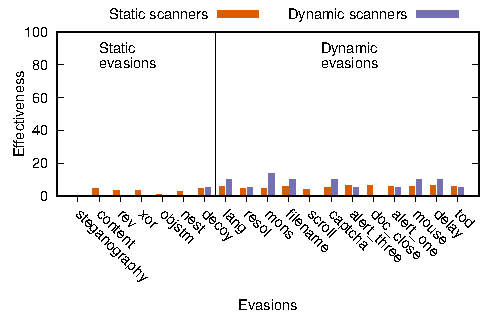
\includegraphics{figures/average-worst-case-counter-eff}
    \caption{Counter-effectiveness for different classes of static and 
    dynamic evasions. The results are averaged over all static
    (red) and dynamic (blue) scanners.}
    \label{fig: worst case counter-eff}
\end{figure}

Figure~\ref{fig: worst case counter-eff} shows the counter-effectiveness of the studied evasions, sorted as in Figure~\ref{fig: best case eff}.
Perhaps surprisingly, most evasions are, at least sometimes, counter-effective.
A likely reason is that some scanners consider the changes of the document caused by the evasions as indicators of malicious intent.
For example, the context-related evasions add some code to the document to check the
current context, and  some scanners may consider this activity to be suspicious.
In fact, all context-related and time-related evasions are counter-effective.
Furthermore, all evasions are counter-effective for at least some static scanners, with the exception of the ``steganography'' evasion.
This evasion's high effectiveness (Figure~\ref{fig: best
  case eff}) and low counter-effectiveness  should concern the developers of scanners.

Although most evasions are sometimes counter-effective, the counter-effectiveness in Figure~\ref{fig: worst case counter-eff} is relatively low compared to the effectiveness of evasions.
Moreover, we observe counter-effectiveness only in a relatively small subset of the studied scanners.
For static scanners, the evasions behave counter-effectively only on McAfee-GW-Edition, Qihoo-360, and Rising.
For dynamic scanners, all counter-effective behavior that we observe is due to DS2.


\subsection{RQ5: Combinations of Evasions}
\label{ss:combinations}

A combination of evasions may be more effective than the individual evasions.
For example, even though some evasions may not be able to bypass a scanner alone, their combination may be able to do so (RQ5).
In the following we discuss the  added effectiveness of
combined dynamic, combined static, and hybrid evasions.
Figure~\ref{fig: added eff} presents the results for combined evasions with more than 0.5\% added effectiveness.
Averaged over all scanners, the added effectiveness of even the most successful combined evasions is relatively low (about 3.2\%).
For some individual scanners, though, we find higher added effectiveness values.
That is, an attacker interested in bypassing a particular scanner could combine evasions suitable for this task.

\begin{figure}[tb]
    \hspace{-.4em}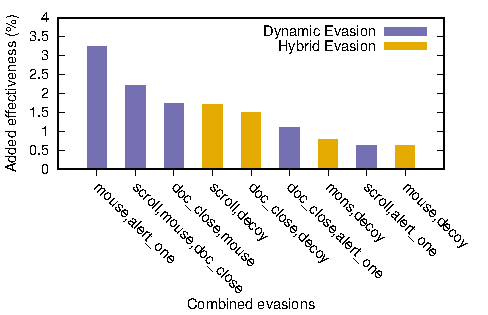
\includegraphics{figures/added-eff}
    \caption{Evasions that have greater than 0.5\% added effectiveness.}
    \label{fig: added eff}
\end{figure}

Interestingly, combining multiple static evasions does not cause any added effectiveness, suggesting that a single static evasion is sufficient to fool scanners susceptible to this kind of evasion.
Furthermore, all combined dynamic evasions in Figure~\ref{fig: added eff} result from combining UI-based evasions, showing that an evasion that requires a more complicated user interaction is more successful.


\subsection{RQ6: Influence of Exploits and Payloads on Evasion Effectiveness}
\label{ss: influence of exploit effectiveness}

The effectiveness of an evasion may depend on the specific exploit or payload used in a malicious document.
For example, consider an exploit that relies on malicious JavaScript and therefore may be detected by scanners that check the JavaScript code in a document.
For such an exploit, a JavaScript-based evasion may work particularly well, because the evasion reduces the chance that scanners identify the document as malicious.
The following studies to what extent the effectiveness of an evasion depends on the exploit or payload used in the malicious document (RQ6).
To this end, we compute the effectiveness of each evasion for the subset of all documents that use a particular exploit or payload.

\subsubsection{Influence of Exploit}

Figure~\ref{figure:toolbutton projection} shows the evasion effectiveness for documents with the ``Toolbutton'' exploit.
The evasions related to JavaScript obfuscation work particularly well, 
since this exploit is based on malicious JavaScript code only, i.e., no other objects, such as fonts or images, are needed.
Many of these evasions are greater than 80\% effective.
The sudden drop in the effectiveness of static and hybrid evasions is also due to the drastically higher success of JavaScript obfuscation-based versus PDF obfuscation-based evasions.

The evasion effectiveness for documents based on the ``Cooltype'' exploit is shown in Figure~\ref{figure:cooltype projection}.
We use the same order of evasions as in Figure~\ref{figure:toolbutton projection} to enable a comparison between the two exploits.
The results show several interesting effects.
First, the most effective evasions for the ``Toolbutton'' exploit reach almost 100\% effectiveness, whereas the peak effectiveness of ``Cooltype''-based documents is only around 75\%.
The reason is that ``Cooltype'' requires both malicious JavaScript code and a malicious font file to be embedded in the PDF.
As a result, none of the static evasions alone is highly effective at hiding ``Cooltype''-based documents.
Second, the effectiveness of evasions based on PDF obfuscation are higher for ``Cooltype'' than for ``Toolbutton'' (the second half of static evasions' bars in the figure).
This result suggests that many scanners identify the exploit by searching for the
malicious font file and thereby make those evasions effective that change the signature of
the PDF document (and hence the signature of the embedded font file).


\subsubsection{Influence of Payload}

With the same approach as exploits, we study the dependence of the evasions on the payload.
We compute the effectiveness of the subset of the samples with each of the three payloads.
In contrast to the exploits, we do not observe any major differences in effectiveness of the evasions.

\medskip
\noindent
Overall, studying the influence of exploits and payloads on the effectiveness of evasions shows that exploits and evasions may influence each other.
Developers of PDF scanners should be aware of this influence when developing anti-evasion techniques, as an attacker might choose suitable evasions depending on how a PDF exploit works.

